\RequirePackage[table]{xcolor}
\documentclass[fonts]{icst}

\usepackage{moreverb}

\usepackage[breaklinks,colorlinks,bookmarksopen,bookmarksnumbered,linkcolor=ICSTblue,citecolor=blue,urlcolor=ICSTblue]{hyperref}
\usepackage{iftex}
\ifPDFTeX\usepackage{breakurl}\fi
\usepackage{doi}
\usepackage{xurl}

\usepackage[utf8]{inputenc}
\usepackage[english]{babel}
\usepackage{amsmath,amssymb,amsthm}
\usepackage{graphicx,flushend}
\usepackage{booktabs}
\usepackage{array}
\usepackage{multirow}
\usepackage{float}
\usepackage{enumitem}
\usepackage{dblfloatfix}
\usepackage{cuted}
\usepackage[hypcap=false]{caption}
\usepackage{adjustbox}
\usepackage{balance}

% ---------------------------------------------------------------- revision helpers
% This file is the first-version manuscript (BiasLN_final.tex) edited in place.
% Text changed in response to the reviews is printed in blue (\revmarktrue);
% set \revmarkfalse for the clean version.
\newif\ifrevmark\revmarktrue
\definecolor{revblue}{RGB}{0,70,200}
\newcommand{\rev}[1]{\ifrevmark{\color{revblue}#1}\else#1\fi}
\newenvironment{revblock}{\ifrevmark\color{revblue}\fi}{}
% \pending{...} marks text whose final wording depends on runs still in progress.
% build.sh with FINAL=1 sets \pendingfalse; any remaining \pending is then an error.
\newif\ifpending\pendingfalse
\newcommand{\pending}[1]{\ifpending\textcolor{red}{[#1]}\else\errmessage{pending text left: #1}\fi}
\IfFileExists{generated/numbers.tex}{% generated by tools/paper_assets.py -- do not edit
\newcommand{\AvgDBal}{0.911}
\newcommand{\StdDBal}{0.000}
\newcommand{\NDBal}{1}
\newcommand{\AvgMBal}{0.954}
\newcommand{\StdMBal}{0.000}
\newcommand{\NMBal}{1}
\newcommand{\AvgFFBal}{0.993}
\newcommand{\StdFFBal}{0.000}
\newcommand{\NFFBal}{1}
\newcommand{\AvgDBiasGate}{0.920}
\newcommand{\StdDBiasGate}{0.000}
\newcommand{\NDBiasGate}{1}
\newcommand{\AvgMBiasGate}{0.958}
\newcommand{\StdMBiasGate}{0.000}
\newcommand{\NMBiasGate}{1}
\newcommand{\AvgFFBiasGate}{0.988}
\newcommand{\StdFFBiasGate}{0.000}
\newcommand{\NFFBiasGate}{1}
\newcommand{\AvgDBiasShift}{0.915}
\newcommand{\StdDBiasShift}{0.000}
\newcommand{\NDBiasShift}{1}
\newcommand{\AvgMBiasShift}{0.960}
\newcommand{\StdMBiasShift}{0.000}
\newcommand{\NMBiasShift}{1}
\newcommand{\AvgFFBiasShift}{0.993}
\newcommand{\StdFFBiasShift}{0.000}
\newcommand{\NFFBiasShift}{1}
\newcommand{\AvgDBiasln}{0.923}
\newcommand{\StdDBiasln}{0.006}
\newcommand{\NDBiasln}{3}
\newcommand{\AvgMBiasln}{0.957}
\newcommand{\StdMBiasln}{0.005}
\newcommand{\NMBiasln}{3}
\newcommand{\AvgFFBiasln}{0.995}
\newcommand{\StdFFBiasln}{0.001}
\newcommand{\NFFBiasln}{3}
\newcommand{\AvgDBiaslnAsy}{0.911}
\newcommand{\StdDBiaslnAsy}{0.000}
\newcommand{\NDBiaslnAsy}{1}
\newcommand{\AvgMBiaslnAsy}{0.970}
\newcommand{\StdMBiaslnAsy}{0.000}
\newcommand{\NMBiaslnAsy}{1}
\newcommand{\AvgFFBiaslnAsy}{0.994}
\newcommand{\StdFFBiaslnAsy}{0.000}
\newcommand{\NFFBiaslnAsy}{1}
\newcommand{\AvgDBitfit}{0.921}
\newcommand{\StdDBitfit}{0.006}
\newcommand{\NDBitfit}{3}
\newcommand{\AvgMBitfit}{0.960}
\newcommand{\StdMBitfit}{0.005}
\newcommand{\NMBitfit}{3}
\newcommand{\AvgFFBitfit}{0.994}
\newcommand{\StdFFBitfit}{0.001}
\newcommand{\NFFBitfit}{3}
\newcommand{\AvgDBitfitLC}{0.915}
\newcommand{\StdDBitfitLC}{0.000}
\newcommand{\NDBitfitLC}{1}
\newcommand{\AvgMBitfitLC}{0.959}
\newcommand{\StdMBitfitLC}{0.000}
\newcommand{\NMBitfitLC}{1}
\newcommand{\AvgFFBitfitLC}{0.995}
\newcommand{\StdFFBitfitLC}{0.000}
\newcommand{\NFFBitfitLC}{1}
\newcommand{\AvgDDepthAToBI}{0.923}
\newcommand{\StdDDepthAToBI}{0.004}
\newcommand{\NDDepthAToBI}{3}
\newcommand{\AvgMDepthAToBI}{0.960}
\newcommand{\StdMDepthAToBI}{0.005}
\newcommand{\NMDepthAToBI}{3}
\newcommand{\AvgFFDepthAToBI}{0.994}
\newcommand{\StdFFDepthAToBI}{0.001}
\newcommand{\NFFDepthAToBI}{3}
\newcommand{\AvgDDepthFirstBC}{0.904}
\newcommand{\StdDDepthFirstBC}{0.000}
\newcommand{\NDDepthFirstBC}{1}
\newcommand{\AvgMDepthFirstBC}{0.946}
\newcommand{\StdMDepthFirstBC}{0.000}
\newcommand{\NMDepthFirstBC}{1}
\newcommand{\AvgFFDepthFirstBC}{0.989}
\newcommand{\StdFFDepthFirstBC}{0.000}
\newcommand{\NFFDepthFirstBC}{1}
\newcommand{\AvgDDepthFirstG}{0.894}
\newcommand{\StdDDepthFirstG}{0.000}
\newcommand{\NDDepthFirstG}{1}
\newcommand{\AvgMDepthFirstG}{0.939}
\newcommand{\StdMDepthFirstG}{0.000}
\newcommand{\NMDepthFirstG}{1}
\newcommand{\AvgFFDepthFirstG}{0.978}
\newcommand{\StdFFDepthFirstG}{0.000}
\newcommand{\NFFDepthFirstG}{1}
\newcommand{\AvgDDepthFisherBCToBI}{0.903}
\newcommand{\StdDDepthFisherBCToBI}{0.000}
\newcommand{\NDDepthFisherBCToBI}{1}
\newcommand{\AvgMDepthFisherBCToBI}{0.945}
\newcommand{\StdMDepthFisherBCToBI}{0.000}
\newcommand{\NMDepthFisherBCToBI}{1}
\newcommand{\AvgFFDepthFisherBCToBI}{0.984}
\newcommand{\StdFFDepthFisherBCToBI}{0.000}
\newcommand{\NFFDepthFisherBCToBI}{1}
\newcommand{\AvgDDepthLastBC}{0.891}
\newcommand{\StdDDepthLastBC}{0.000}
\newcommand{\NDDepthLastBC}{1}
\newcommand{\AvgMDepthLastBC}{0.939}
\newcommand{\StdMDepthLastBC}{0.000}
\newcommand{\NMDepthLastBC}{1}
\newcommand{\AvgFFDepthLastBC}{0.985}
\newcommand{\StdFFDepthLastBC}{0.000}
\newcommand{\NFFDepthLastBC}{1}
\newcommand{\AvgDDepthLastG}{0.885}
\newcommand{\StdDDepthLastG}{0.000}
\newcommand{\NDDepthLastG}{1}
\newcommand{\AvgMDepthLastG}{0.945}
\newcommand{\StdMDepthLastG}{0.000}
\newcommand{\NMDepthLastG}{1}
\newcommand{\AvgFFDepthLastG}{0.969}
\newcommand{\StdFFDepthLastG}{0.000}
\newcommand{\NFFDepthLastG}{1}
\newcommand{\AvgDDepthMidBC}{0.920}
\newcommand{\StdDDepthMidBC}{0.000}
\newcommand{\NDDepthMidBC}{2}
\newcommand{\AvgMDepthMidBC}{0.964}
\newcommand{\StdMDepthMidBC}{0.005}
\newcommand{\NMDepthMidBC}{2}
\newcommand{\AvgFFDepthMidBC}{0.992}
\newcommand{\StdFFDepthMidBC}{0.001}
\newcommand{\NFFDepthMidBC}{2}
\newcommand{\AvgDEffort}{0.911}
\newcommand{\StdDEffort}{0.002}
\newcommand{\NDEffort}{3}
\newcommand{\AvgMEffort}{0.960}
\newcommand{\StdMEffort}{0.006}
\newcommand{\NMEffort}{3}
\newcommand{\AvgFFEffort}{0.991}
\newcommand{\StdFFEffort}{0.001}
\newcommand{\NFFEffort}{3}
\newcommand{\AvgDFullft}{0.823}
\newcommand{\StdDFullft}{0.000}
\newcommand{\NDFullft}{1}
\newcommand{\AvgMFullft}{0.819}
\newcommand{\StdMFullft}{0.000}
\newcommand{\NMFullft}{1}
\newcommand{\AvgFFFullft}{0.986}
\newcommand{\StdFFFullft}{0.000}
\newcommand{\NFFFullft}{1}
\newcommand{\AvgDGend}{0.925}
\newcommand{\StdDGend}{0.002}
\newcommand{\NDGend}{3}
\newcommand{\AvgMGend}{0.966}
\newcommand{\StdMGend}{0.002}
\newcommand{\NMGend}{3}
\newcommand{\AvgFFGend}{0.986}
\newcommand{\StdFFGend}{0.001}
\newcommand{\NFFGend}{3}
\newcommand{\AvgDLinprobe}{0.774}
\newcommand{\StdDLinprobe}{0.000}
\newcommand{\NDLinprobe}{1}
\newcommand{\AvgMLinprobe}{0.793}
\newcommand{\StdMLinprobe}{0.000}
\newcommand{\NMLinprobe}{1}
\newcommand{\AvgFFLinprobe}{0.829}
\newcommand{\StdFFLinprobe}{0.000}
\newcommand{\NFFLinprobe}{1}
\newcommand{\AvgDLnBeta}{0.914}
\newcommand{\StdDLnBeta}{0.000}
\newcommand{\NDLnBeta}{1}
\newcommand{\AvgMLnBeta}{0.958}
\newcommand{\StdMLnBeta}{0.000}
\newcommand{\NMLnBeta}{1}
\newcommand{\AvgFFLnBeta}{0.985}
\newcommand{\StdFFLnBeta}{0.000}
\newcommand{\NFFLnBeta}{1}
\newcommand{\AvgDLnGamma}{0.914}
\newcommand{\StdDLnGamma}{0.000}
\newcommand{\NDLnGamma}{1}
\newcommand{\AvgMLnGamma}{0.961}
\newcommand{\StdMLnGamma}{0.000}
\newcommand{\NMLnGamma}{1}
\newcommand{\AvgFFLnGamma}{0.984}
\newcommand{\StdFFLnGamma}{0.000}
\newcommand{\NFFLnGamma}{1}
\newcommand{\AvgDLnLC}{0.921}
\newcommand{\StdDLnLC}{0.000}
\newcommand{\NDLnLC}{1}
\newcommand{\AvgMLnLC}{0.959}
\newcommand{\StdMLnLC}{0.000}
\newcommand{\NMLnLC}{1}
\newcommand{\AvgFFLnLC}{0.987}
\newcommand{\StdFFLnLC}{0.000}
\newcommand{\NFFLnLC}{1}
\newcommand{\AvgDLora}{0.901}
\newcommand{\StdDLora}{0.000}
\newcommand{\NDLora}{1}
\newcommand{\AvgMLora}{0.961}
\newcommand{\StdMLora}{0.000}
\newcommand{\NMLora}{1}
\newcommand{\AvgFFLora}{0.993}
\newcommand{\StdFFLora}{0.000}
\newcommand{\NFFLora}{1}
\newcommand{\AvgDLoraNolC}{0.909}
\newcommand{\StdDLoraNolC}{0.000}
\newcommand{\NDLoraNolC}{1}
\newcommand{\AvgMLoraNolC}{0.948}
\newcommand{\StdMLoraNolC}{0.000}
\newcommand{\NMLoraNolC}{1}
\newcommand{\AvgFFLoraNolC}{0.995}
\newcommand{\StdFFLoraNolC}{0.000}
\newcommand{\NFFLoraNolC}{1}
\newcommand{\AvgDProto}{0.907}
\newcommand{\StdDProto}{0.000}
\newcommand{\NDProto}{1}
\newcommand{\AvgMProto}{0.958}
\newcommand{\StdMProto}{0.000}
\newcommand{\NMProto}{1}
\newcommand{\AvgFFProto}{0.991}
\newcommand{\StdFFProto}{0.000}
\newcommand{\NFFProto}{1}
\newcommand{\AvgDRaAll}{0.921}
\newcommand{\StdDRaAll}{0.001}
\newcommand{\NDRaAll}{2}
\newcommand{\AvgMRaAll}{0.960}
\newcommand{\StdMRaAll}{0.000}
\newcommand{\NMRaAll}{2}
\newcommand{\AvgFFRaAll}{0.992}
\newcommand{\StdFFRaAll}{0.000}
\newcommand{\NFFRaAll}{2}
\newcommand{\AvgDRaFake}{0.923}
\newcommand{\StdDRaFake}{0.000}
\newcommand{\NDRaFake}{1}
\newcommand{\AvgMRaFake}{0.962}
\newcommand{\StdMRaFake}{0.000}
\newcommand{\NMRaFake}{1}
\newcommand{\AvgFFRaFake}{0.992}
\newcommand{\StdFFRaFake}{0.000}
\newcommand{\NFFRaFake}{1}
\newcommand{\AvgDRaGate}{0.917}
\newcommand{\StdDRaGate}{0.000}
\newcommand{\NDRaGate}{1}
\newcommand{\AvgMRaGate}{0.953}
\newcommand{\StdMRaGate}{0.000}
\newcommand{\NMRaGate}{1}
\newcommand{\AvgFFRaGate}{0.986}
\newcommand{\StdFFRaGate}{0.000}
\newcommand{\NFFRaGate}{1}
\newcommand{\AvgDRaProto}{0.918}
\newcommand{\StdDRaProto}{0.000}
\newcommand{\NDRaProto}{1}
\newcommand{\AvgMRaProto}{0.960}
\newcommand{\StdMRaProto}{0.000}
\newcommand{\NMRaProto}{1}
\newcommand{\AvgFFRaProto}{0.993}
\newcommand{\StdFFRaProto}{0.000}
\newcommand{\NFFRaProto}{1}
\newcommand{\AvgDRaReal}{0.927}
\newcommand{\StdDRaReal}{0.004}
\newcommand{\NDRaReal}{2}
\newcommand{\AvgMRaReal}{0.961}
\newcommand{\StdMRaReal}{0.001}
\newcommand{\NMRaReal}{2}
\newcommand{\AvgFFRaReal}{0.991}
\newcommand{\StdFFRaReal}{0.000}
\newcommand{\NFFRaReal}{2}
\newcommand{\AvgDRaRealLAD}{0.922}
\newcommand{\StdDRaRealLAD}{0.000}
\newcommand{\NDRaRealLAD}{1}
\newcommand{\AvgMRaRealLAD}{0.968}
\newcommand{\StdMRaRealLAD}{0.000}
\newcommand{\NMRaRealLAD}{1}
\newcommand{\AvgFFRaRealLAD}{0.993}
\newcommand{\StdFFRaRealLAD}{0.000}
\newcommand{\NFFRaRealLAD}{1}
\newcommand{\AvgDRaRealLD}{0.913}
\newcommand{\StdDRaRealLD}{0.000}
\newcommand{\NDRaRealLD}{1}
\newcommand{\AvgMRaRealLD}{0.936}
\newcommand{\StdMRaRealLD}{0.000}
\newcommand{\NMRaRealLD}{1}
\newcommand{\AvgFFRaRealLD}{0.982}
\newcommand{\StdFFRaRealLD}{0.000}
\newcommand{\NFFRaRealLD}{1}
}{}
\IfFileExists{generated/drift_numbers.tex}{% generated by tools/feature_figs.py -- do not edit
\newcommand{\FisherClip}{0.02}
\newcommand{\FisherEffort}{0.07}
\newcommand{\FisherGend}{0.04}
\newcommand{\FisherBiasln}{0.40}
}{}
\newcommand{\num}[1]{\ifcsname #1\endcsname\csname #1\endcsname\else\textcolor{red}{??}\fi}
\newtheorem{proposition}{Proposition}

\newcommand\BibTeX{{\rmfamily B\kern-.05em \textsc{i\kern-.025em b}\kern-.08emT\kern-.1667em\lower.7ex\hbox{E}\kern-.125emX}}
\def\volumeyear{2024}
\journalname{XXXXXX}
\articletype{Research Article}
\setcounter{page}{01}
\def\volumeyear{XXXX}
\def\volumenumber{XX}
\def\issuemonth{XX-XX}
\def\issuenumber{X}
\def\articleid{XX}
\def\copyrightholder{Xuan-Huy Dinh\textit{ et al.}, licensed to ICST}
\copyrightnote{This is an open access article distributed under the terms of the Creative Commons Attribution license (\url{http://creativecommons.org/licenses/by/3.0/}), which permits unlimited use, distribution and reproduction in any medium so long as the original work is properly cited.}
\def\articledoi{10.4108/XX.X.X.XX}
\received{XXXX}
\accepted{XXXX}
\published{XXXX}

\begin{document}

\runningheads{}{}

\title{BiasLN: Efficient Tuning for Generalizable Deepfake Detection Across Benchmarks}

\author{Xuan-Huy Dinh,\ Minh-Duc Vu,\ Thanh-Quan Phung-Le,\ Duc-Thinh Nguyen,\ Van-Dung Hoang\fnoteref{1}}

\address{
    Faculty of Information Technology\\
    Ho Chi Minh City University of Technology and Engineering (HCMUTE)\\
    Ho Chi Minh City, Vietnam
}

\abstract{
Achieving robust generalization to unseen manipulation techniques remains a key challenge for existing detection models. Although Parameter-Efficient Fine-Tuning (PEFT) holds significant promise, existing approaches often rely on complex adaptation schemes that can disrupt pre-trained representations or lead to overfitting. To address this issue, we introduce BiasLN, a simple PEFT strategy. Instead of incorporating additional modules that increase model complexity, we fine-tune only the bias terms and LayerNorm parameters of a pre-trained image encoder. \rev{We show that this parameter set is the complete per-channel affine adaptation of the encoder: a LayerNorm shift is exactly a tied update of the following biases, the key biases receive no gradient, and the LayerNorm scales are the only multiplicative component.} This design preserves the core visual knowledge learned during pre-training while enhancing the model's ability to capture subtle manipulation artifacts. \rev{All methods are re-trained under one protocol that selects every checkpoint on the FaceForensics++ validation split, disjoint from all test sets, and results are reported over several seeds. Under this protocol BiasLN reaches an average video AUC of \num{AvgDBiasln} on four unseen datasets and \num{AvgMBiasln} on seven unseen face-swapping methods, on par with re-trained GenD on the unseen datasets (\num{AvgDGend}) and about one point below it on the unseen methods (\num{AvgMGend}), above Effort (\num{AvgDEffort}), with the highest in-domain accuracy, without auxiliary losses and without any additional inference cost.} The proposed approach shows that a simple parameter-efficient design \rev{is a strong baseline} for generalizable deepfake detection.
}

\keywords{Deepfake detection, parameter-efficient fine-tuning, \rev{bias tuning,} LayerNorm tuning}

\fnotetext[1]{Corresponding author. Email: \email{dunghv@hcmute.edu.vn}}

\maketitle

\section{Introduction}
The rapid growth of generative models, especially GANs~\cite{goodfellow2020gan} and diffusion models~\cite{yang2022diffusion}, has drawn significant attention in recent years. However, these advances also introduce serious risks, particularly their potential misuse for creating realistic fake face videos. Therefore, developing effective forgery detection models is essential.

Traditional detectors often rely on CNNs or frequency-domain artifacts. However, modern generative methods continue to minimize these local errors, making them increasingly difficult to detect using standard approaches.
This shift has led the field toward vision foundation models like CLIP and DINO~\cite{radford2021clip_vitl,caron2021emerging}.
These models offer robust, global representations that have already shown significant promise in ``universal'' detection tasks~\cite{ojha2023universal}.

However, fully fine-tuning these large models often \rev{distorts their pre-trained features}, which reduces their generalization ability~\cite{kumar2022finetuning}.
To address this issue, Parameter-Efficient Fine-Tuning (PEFT) has emerged as a promising alternative. Recent methods such as Effort~\cite{yan2025effort} and GenD~\cite{yermakov2025gend} achieve strong cross-dataset performance by adapting models in different spaces, such as weight space or feature space.
Despite their effectiveness, these approaches introduce additional complexity, raising the question of whether such designs are truly necessary for robust deepfake detection.

We introduce BiasLN, a simple parameter-efficient fine-tuning strategy that updates only the bias terms and LayerNorm affine parameters of a pre-trained vision encoder while keeping all other weights frozen. This design provides sufficient adaptation capacity while preserving pre-trained knowledge. \rev{Bias tuning~\cite{benzaken2022bitfit} and LayerNorm tuning~\cite{wang2022ln,yermakov2025gend} have each been used before; our aim is to make precise what their combination can express and to measure, under a protocol that never uses test data for model selection, how it compares with recent detectors.}

We evaluate BiasLN under in-domain, cross-dataset and cross-method settings. Following the protocol of Effort~\cite{yan2025effort}, the model is trained on a single source dataset \rev{and evaluated on four unseen datasets as well as seven single-method benchmarks. Every checkpoint, including those of the re-trained baselines, is selected on the validation split of the source dataset only, and results are reported as the mean and standard deviation over several random seeds.}

In summary, our key contributions are as follows:
\begin{enumerate}
    \item \textbf{A simple \rev{method with an analysis of what it tunes}:} BiasLN updates only the bias and LayerNorm parameters of a vision encoder. \rev{We show that a LayerNorm shift is a tied bias update and that the key biases receive no gradient, so BiasLN is the complete per-channel affine adaptation of the frozen encoder, and the LayerNorm scales are what it adds to bias tuning.}

    \item \textbf{Extensive generalization evaluation:} Extensive experiments on \rev{four} unseen datasets and seven single-method benchmarks \rev{show that BiasLN reaches the highest in-domain accuracy and cross-dataset accuracy on par with GenD and above Effort, and cross-method accuracy about one point below GenD, without auxiliary losses or inference overhead.}

    \item \rev{\textbf{A controlled, leakage-free comparison:} BiasLN, GenD, Effort, LoRA, bias-only and LayerNorm-only tuning, a linear probe and full fine-tuning are re-trained in one pipeline with the same data and the same checkpoint-selection rule; ablations change one factor at a time, and training and inference costs are measured on the same GPU.}
\end{enumerate}
At a high level, BiasLN starts from a frozen CLIP vision encoder and updates only its bias and LayerNorm parameters, while keeping all other weights fixed.
A lightweight classification head is trained on top of the adapted features for real/fake prediction.

The official source code \rev{is available} at \href{https://github.com/ducthinh4477/BiasLN}{\rev{https://github.com/ducthinh4477/BiasLN}}.

\section{Related Work}

Generalizable deepfake detection remains difficult because many detectors overfit to dataset-specific artifacts. Early methods mainly relied on CNNs, frequency cues, or reconstruction signals to detect facial manipulations~\cite{rossler2019ff,qian2020frequency,luo2021srm,liu2021spsl,cao2022recce,badr2025wavit}. \rev{Data-centric methods synthesize training forgeries~\cite{shiohara2022sbi,chen2022sladd,lin2024cdfa}, augment the latent space~\cite{yan2024latent} or disentangle forgery-specific features~\cite{yan2023ucf,huang2023iid}.} Although effective in-domain, these approaches often degrade on unseen forgeries because they depend heavily on low-level or method-specific artifacts.

To address this limitation, recent research has expanded from facial manipulation detection to broader AI-generated image detection and increasingly adopts vision foundation models, particularly CLIP, to improve cross-domain generalization~\cite{ojha2023universal,cui2025forada,yan2025effort,yermakov2025gend}. These methods can be grouped by their adaptation strategies. \rev{Forensics Adapter (ForAda)}~\cite{cui2025forada} introduces a lightweight parallel adapter network to explicitly learn blending boundaries alongside the original vision-language model. Effort~\cite{yan2025effort} instead operates in parameter space through Singular Value Decomposition (SVD), freezing principal components and fine-tuning residual low-rank components to preserve pre-trained knowledge. Building on this parameter-efficient direction, GenD~\cite{yermakov2025gend} further reduces the trainable footprint by updating only LayerNorm parameters and complementing this design with feature-space objectives, including a uniform loss on the $L_2$ hypersphere and an alignment loss that pulls same-class samples closer together\rev{~\cite{wang2020alignment}. Its ablation also reports that bias tuning reaches an average similar to LayerNorm tuning. BPL~\cite{xu2026bpl}, concurrent with this work, tunes only biases and learns from mined real--fake pairs.}

\rev{In parameter-efficient tuning more generally, BitFit~\cite{benzaken2022bitfit} tunes only the biases of a transformer and observes that the query and intermediate MLP biases alone recover most of the accuracy, and Namazifar et al.~\cite{namazifar2023bias} prove that the key bias of dot-product attention has no effect on the output. Tuning only the normalization layers is also expressive~\cite{giannou2023layernorm,wang2022ln,valizadeh2024layernorm}.}
Compared with these approaches, BiasLN simply tunes only bias and LayerNorm parameters, avoiding the need for additional architectural branches or multi-objective training losses\rev{, and Sec.~\ref{sec:analysis} makes precise how the two parameter groups overlap.}

\section{Methodology}
\label{sec:method}

We propose \textbf{BiasLN}, a simple parameter-efficient fine-tuning framework for generalizable deepfake detection. BiasLN freezes the pre-trained CLIP visual encoder and tunes only bias and LayerNorm affine parameters, preserving the pre-trained feature space while adapting the model to binary real/fake classification. Motivated by Effort~\cite{yan2025effort} and related PEFT methods such as BitFit~\cite{benzaken2022bitfit} and LayerNorm tuning~\cite{wang2022ln}, this design aims to improve cross-domain generalization with only a small number of trainable parameters. \rev{Figure~\ref{fig:model} gives an overview.}

\begin{figure}[H]
    \centering
    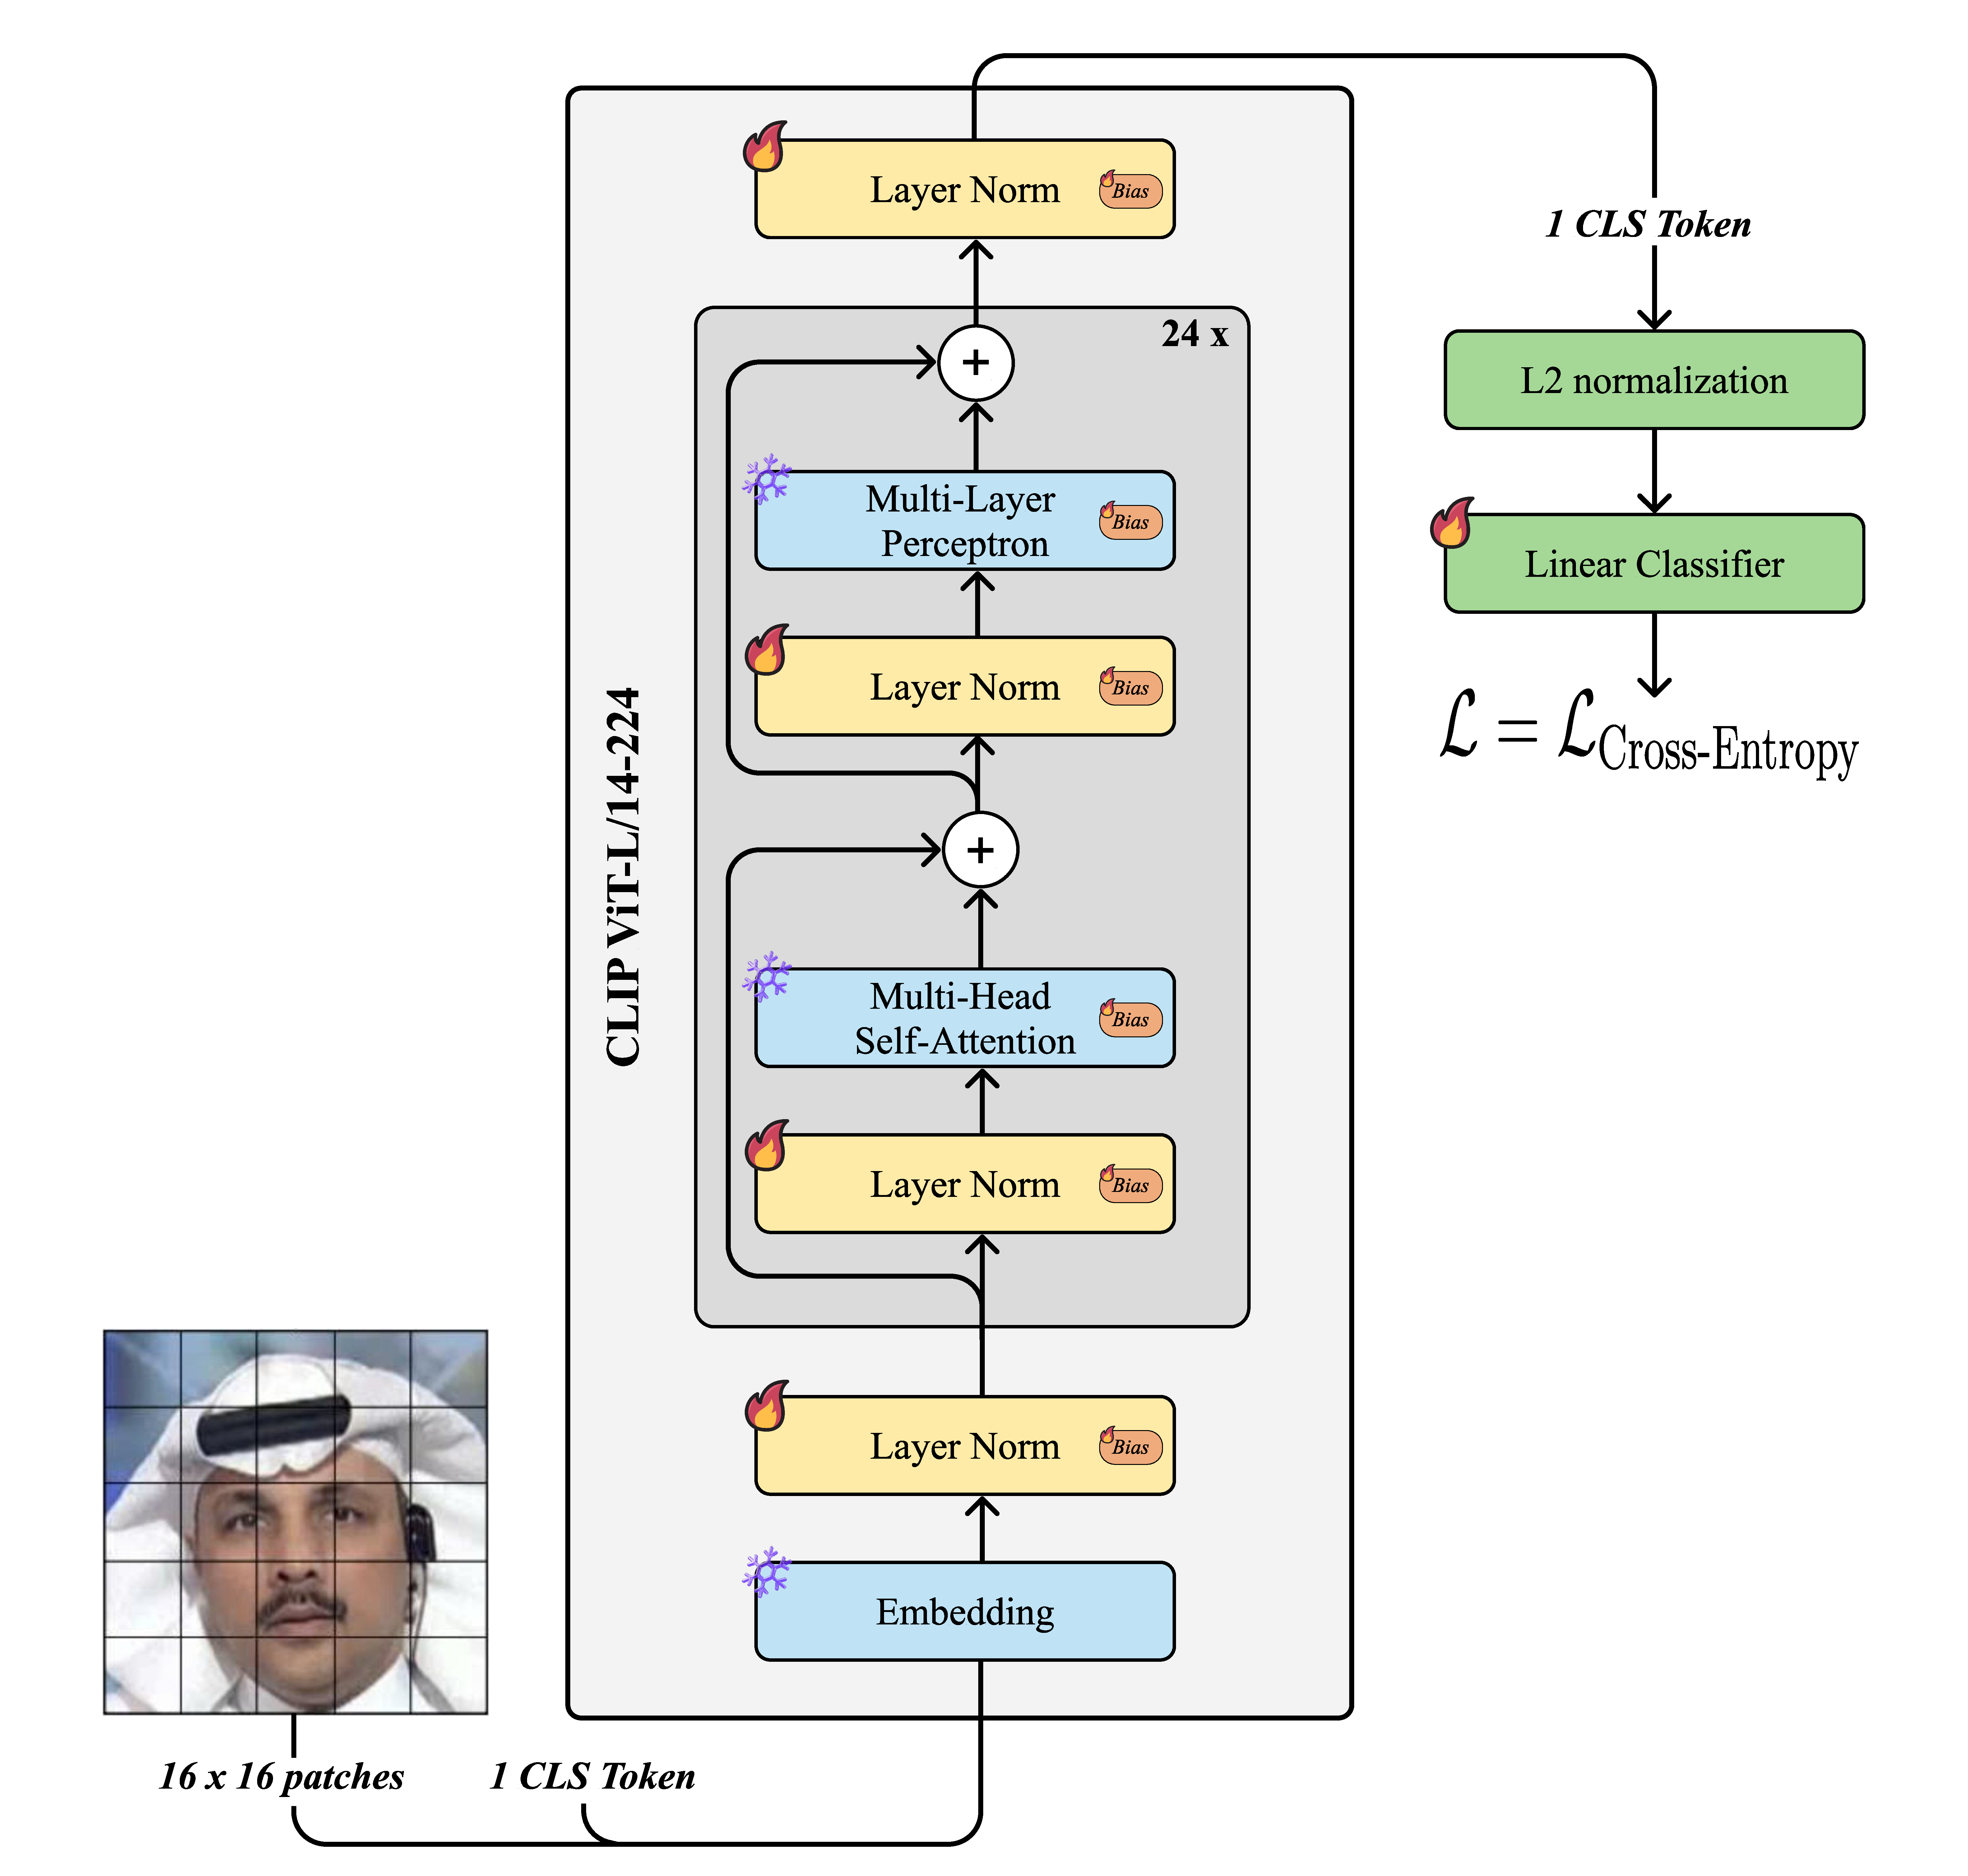
\includegraphics[width=\linewidth]{figs/biasln_overview.pdf}
    \caption{Overview of BiasLN.
The CLIP ViT-L/14 backbone is kept frozen except for bias terms and LayerNorm parameters, and the extracted features are passed to a lightweight classifier for deepfake detection.}
    \label{fig:model}
\end{figure}

\subsection{Feature Extractor}

Given an input image $\mathbf{x}$, the CLIP visual encoder~\cite{radford2021clip_vitl} extracts a global feature representation
\begin{equation}
\mathbf{f} = g_{\theta}(\mathbf{x}),
\end{equation}
where $\mathbf{f} \in \mathbb{R}^{1024}$ denotes the output of the CLS token \rev{after the final LayerNorm}.
To \rev{limit the distortion of the pre-trained features}, \rev{all weight matrices} of $g_{\theta}$---\rev{the} attention \rev{projections} and \rev{the} feed-forward weights---remain frozen during training.
Adaptation to the deepfake detection task is therefore delegated to a highly constrained parameter-efficient fine-tuning strategy.

\subsection{Parameter-Efficient Fine-Tuning (PEFT) Strategy}
\label{sec:peft}

Rather than fine-tuning the full CLIP backbone, we adopt a minimal parameter update scheme that we term \textbf{BiasLN}.
This strategy combines two lightweight tuning mechanisms to preserve the structural integrity of the pre-trained model while still enabling effective adaptation to the target domain.

\paragraph{BitFit (Bias-only Tuning).}
Introduced by Ben Zaken et al.~\cite{benzaken2022bitfit}, BitFit is a sparse fine-tuning paradigm that restricts trainable parameters exclusively to the bias terms of the network.
Formally, for a standard linear projection layer receiving an input $\mathbf{u} \in \mathbb{R}^{d}$, the output $\mathbf{h} \in \mathbb{R}^{k}$ is computed as
\begin{equation}
    \mathbf{h} = \mathbf{W}\mathbf{u} + \mathbf{b},
\end{equation}
where $\mathbf{W} \in \mathbb{R}^{k \times d}$ is the weight matrix and $\mathbf{b} \in \mathbb{R}^{k}$ is the bias vector.
In traditional full fine-tuning, both $\mathbf{W}$ and $\mathbf{b}$ are updated.
Under the BitFit protocol, the weight matrix is frozen to its pre-trained state, and only the bias vector is optimized:
\begin{equation}
    \mathbf{h} = \mathbf{W}_{\text{pt}}\mathbf{u} + \mathbf{b}_{\text{tuned}}.
\end{equation}
In our framework, we apply this bias-only tuning rule \rev{to all six linear layers of each of the 24 transformer blocks (the query, key, value and output projections of self-attention and the two MLP layers fc1 and fc2)}.
As a result, the domain-specific adaptation required for deepfake detection is largely absorbed into the bias parameters, while the \rev{weight matrices} of the backbone remain intact.

\paragraph{Layer Normalization (LayerNorm) Tuning.}
Complementary to the bias vectors, the LayerNorm blocks play a central role in feature scaling and shifting.
For a given intermediate representation $\mathbf{u} \in \mathbb{R}^{d}$, the LayerNorm operation is defined as
\begin{equation}
    \mathrm{LN}(\mathbf{u}) = \boldsymbol{\gamma} \odot \frac{\mathbf{u} - \mu}{\sqrt{\sigma^2 + \epsilon}} + \boldsymbol{\beta},
\end{equation}
where $\mu$ and $\sigma^2$ denote the empirical mean and variance of $\mathbf{u}$ across the feature dimension, $\epsilon$ is a small constant for numerical stability, $\odot$ denotes element-wise multiplication, and $\boldsymbol{\gamma}, \boldsymbol{\beta} \in \mathbb{R}^{d}$ are the learnable affine scale and shift parameters.

Prior work has shown that these affine parameters provide strong task-adaptive capacity in pre-trained models~\cite{wang2022ln,giannou2023layernorm}.
Building on this motivation and following the efficient adaptation paradigm of GenD~\cite{yermakov2025gend}, we restrict gradient updates in LayerNorm blocks solely to these affine components.
By optimizing only $\boldsymbol{\gamma}$ and $\boldsymbol{\beta}$, the model can recalibrate the statistical distribution of the pre-trained features to better align with the deepfake detection domain, while keeping the backbone computation unchanged.

\rev{Altogether BiasLN tunes 323{,}584 encoder parameters (0.107\% of the 303M parameters of the encoder): 272{,}384 bias and LayerNorm-shift parameters and 51{,}200 LayerNorm scales. Table~\ref{tab:budget} lists the budgets of the schemes compared in this paper.}

\begin{table}[H]
\centering
\caption{\rev{Trainable backbone parameters of the tuning schemes on CLIP ViT-L/14 (303.18M parameters). The classifier adds 2{,}050 parameters to every variant.}}
\label{tab:budget}
\footnotesize
\resizebox{\columnwidth}{!}{%
\begin{tabular}{l r r}
\toprule
\textbf{Scheme} & \textbf{Parameters} & \textbf{\% of encoder} \\
\midrule
LayerNorm $\boldsymbol{\gamma},\boldsymbol{\beta}$ (as GenD) & 102{,}400 & 0.034 \\
Biases incl.\ LN $\boldsymbol{\beta}$ (BitFit) & 272{,}384 & 0.090 \\
BitFit + LN $\boldsymbol{\gamma}$ (BiasLN) & 323{,}584 & 0.107 \\
Effort (rank-1 residual of $q,k,v,o$) & 196{,}608 & 0.065 \\
LoRA, $r{=}8$ on $q,v$ & 786{,}432 & 0.259 \\
\bottomrule
\end{tabular}}
\end{table}

\begin{revblock}
\paragraph{What BiasLN can express.}
\label{sec:analysis}
Two simple facts clarify how the two parameter groups overlap.

\begin{proposition}[Key bias is redundant~\cite{namazifar2023bias}]
\label{prop:key}
In softmax attention with scores $s_{ij}=\mathbf{q}_i^\top(\mathbf{W}_k\mathbf{u}_j+\mathbf{b}_k)/\sqrt{d}$, the term $\mathbf{q}_i^\top\mathbf{b}_k/\sqrt{d}$ is the same for every key $j$ and cancels in the softmax. The attention output therefore does not depend on $\mathbf{b}_k$, and $\partial\mathcal{L}/\partial\mathbf{b}_k=\mathbf{0}$.
\end{proposition}

\begin{proposition}[LayerNorm shift is a tied bias update]
\label{prop:fold}
In a pre-norm block, changing the shift of the first LayerNorm by $\Delta\boldsymbol{\beta}$ changes the query, key and value outputs exactly as changing their biases by $(\mathbf{W}_q\Delta\boldsymbol{\beta},\mathbf{W}_k\Delta\boldsymbol{\beta},\mathbf{W}_v\Delta\boldsymbol{\beta})$, because $\mathbf{W}(\boldsymbol{\gamma}\odot\hat{\mathbf{u}}+\boldsymbol{\beta}+\Delta\boldsymbol{\beta})+\mathbf{b}=\mathbf{W}(\boldsymbol{\gamma}\odot\hat{\mathbf{u}}+\boldsymbol{\beta})+(\mathbf{b}+\mathbf{W}\Delta\boldsymbol{\beta})$. Likewise, the shift of the second LayerNorm acts as the bias update $\mathbf{W}_{\mathrm{fc1}}\Delta\boldsymbol{\beta}$ of fc1.
\end{proposition}

We verified numerically that the key-bias gradients of our model are zero (unit test in the released code). By Proposition~\ref{prop:fold}, LayerNorm shift tuning is contained in bias tuning, and the scales $\boldsymbol{\gamma}$ are the only per-channel \emph{multiplicative} parameters of the encoder. BiasLN therefore covers the complete per-channel affine adaptation of the frozen network: every additive shift (biases) and every per-channel rescaling of normalized activations (LayerNorm scales), and nothing that changes the weight matrices. Because all three schemes act mainly through shifts of pre-activations, bias tuning, LayerNorm tuning and BiasLN are expected to behave similarly, and the scales are what distinguishes BiasLN from bias tuning; Sec.~\ref{sec:ablation} examines this empirically.
\end{revblock}

\vspace{0.5em}
\noindent \textbf{Summary of BiasLN.}
By combining BitFit and LayerNorm tuning with a newly initialized classification head, \textbf{BiasLN} preserves the expressive power of the frozen backbone while acquiring sufficient flexibility to distinguish real images from diverse unseen manipulation artifacts.

\subsection{Classification Head and Training Objective}

The $L_2$-normalized CLS representation is used as the input to a linear binary classifier.
Concretely, the 1024-dimensional feature vector is normalized as
\begin{equation}
\tilde{\mathbf{f}} = \frac{\mathbf{f}}{\lVert \mathbf{f} \rVert_2},
\end{equation}
and the prediction head is defined as
\begin{equation}
\rev{\mathbf{z} = h_{\phi}(\tilde{\mathbf{f}}) = \mathbf{W}_h\tilde{\mathbf{f}}+\mathbf{b}_h,}
\end{equation}
where $h_{\phi}$ is a trainable linear head and \rev{$\mathbf{z} \in \mathbb{R}^2$ denotes the logits for the real ($y=0$) and fake ($y=1$) classes, with $p_{i,c}=\mathrm{softmax}(\mathbf{z}_i)_c$; the fake probability $p_{i,1}$ is the detection score.}
The model is trained using class-weighted cross-entropy with label smoothing:
\begin{equation}
\rev{\begin{aligned}
\mathcal{L}_{\mathrm{ce}}&=\frac{\sum_{i=1}^{N}\sum_{c\in\{0,1\}}-\,w_c\,\tilde{y}_{i,c}\log p_{i,c}}{\sum_{i=1}^{N}w_{y_i}},\\
\tilde{y}_{i,c}&=(1-\alpha)\,\mathbb{1}[c=y_i]+\tfrac{\alpha}{2},
\end{aligned}}
\label{eq:ce}
\end{equation}
\rev{where $N$ is the batch size, $w_0=1$ (real) and $w_1=2$ (fake) are the class weights that penalize errors on the fake class more strongly, and $\alpha=0.1$ is the label-smoothing factor that prevents overconfident predictions. The normalization by $\sum_i w_{y_i}$ is the convention of PyTorch's \texttt{CrossEntropyLoss}.}

This simple objective is consistent with the overall philosophy of BiasLN: effective generalization can be obtained using minimal parameter adaptation\rev{, without auxiliary losses}.

\subsection{Training and Data Setup}
\label{sec:impl}

Our proposed model BiasLN is trained on the FaceForensics++ (FF++) dataset under the c23 compression setting and evaluated under cross-dataset and cross-method protocols.

\noindent\textbf{Data Preprocessing.}\par
We follow the standard dataset preprocessing protocol proposed in DeepfakeBench~\cite{yan2023deepfakebench}, which consists of the following steps:
\begin{itemize}[leftmargin=*, topsep=2pt, itemsep=2pt, label=--]
    \item Sample 32 frames evenly from each video.
    \item Extract the largest face in each frame using RetinaFace~\cite{deng2020retinaface}.
    \item Align the detected face using the predicted facial landmarks.
    \item Compute the bounding box for the aligned face.
    \item Enlarge the bounding box by a factor of $1.3\times$.
    \item Crop the face region and resize it to $224 \times 224$.
    \item Save the processed image in lossless format.
\end{itemize}
\rev{For training, 8 evenly spaced frames of every video are used; at test time all 32 frames are scored.}

\noindent\textbf{Data Augmentation.}\par
We enable data augmentation during training and follow the DeepfakeBench~\cite{yan2023deepfakebench} pipeline, similar to other state-of-the-art detectors implemented with the \texttt{Albumentations} library.
The training images are augmented using \rev{the following operations, each applied with probability 0.5}:
\begin{itemize}[leftmargin=*, topsep=2pt, itemsep=2pt, label=--]
    \item Horizontal flipping,
    \item Random rotation (range $[-10, 10]$ degrees),
    \item Gaussian blur (kernel range $[3, 7]$),
    \item \rev{One of} brightness/contrast adjustment (range $[-0.1, 0.1]$)\rev{, FancyPCA, or hue/saturation jitter},
    \item JPEG compression simulation (quality range $[40, 100]$).
\end{itemize}
These augmentations improve robustness to appearance variation, blur, compression artifacts, and the distribution shifts commonly observed in deepfake benchmarks.

\noindent\textbf{Training Configuration and Optimization.}\par
BiasLN is trained for 10 epochs with a batch size of 32 on \rev{one NVIDIA A100-40GB GPU with bfloat16 autocast}.
We use the Adam optimizer with $\beta_1 = 0.9$, $\beta_2 = 0.999$, an initial learning rate of $3 \times 10^{-4}$, and zero weight decay.
The learning rate follows a cosine annealing schedule with $T_{\max}=10$ and a minimum learning rate of $1 \times 10^{-5}$.
\rev{The checkpoint with the highest frame-level AUC on the FF++ validation split is kept (Sec.~\ref{sec:selection}).}

The model is optimized with \rev{the} class-weighted cross-entropy \rev{of Eq.~\eqref{eq:ce}}. To mitigate class imbalance, the fake class is assigned a larger penalty with $w_{\mathrm{fake}}:w_{\mathrm{real}} = 2:1$, and label smoothing with $\alpha = 0.1$ is applied to prevent overconfident predictions.

\section{Experiments}
\subsection{Datasets}
\label{sec:datasets}
\label{sec:protocol}

Our proposed model BiasLN \rev{is} evaluated in three evaluation protocols: \textit{in-domain}, \textit{cross-dataset}, and \textit{cross-method}.
Table~\ref{tab:datasets} summarizes the datasets, their roles, and the number of forgery methods.
Here, \textbf{NoGenMethod} denotes the number of forgery generation methods in each dataset.

\begin{table}[H]
  \centering
  \caption{Datasets used for training and evaluation.
NoGenMethod denotes the number of forgery methods in each dataset.}
  \label{tab:datasets}
  \small
  \setlength{\tabcolsep}{2pt}
  \renewcommand{\arraystretch}{1.1}
  \resizebox{\columnwidth}{!}{
  \begin{tabular}{@{} l c c c >{\raggedright\arraybackslash} m{0.45\columnwidth} @{}}
    \toprule
    \raisebox{0.6\normalbaselineskip}{\textbf{Dataset}} &
    \raisebox{0.6\normalbaselineskip}{\textbf{Year}} &
    \raisebox{0.6\normalbaselineskip}{\textbf{Role}} &
    \multicolumn{1}{c}{\textbf{\shortstack[c]{NoGen-\\Method}}} &
    \multicolumn{1}{c@{}}{\raisebox{0.6\normalbaselineskip}{\textbf{Description}}} \\
    \midrule
    \textbf{FF++}~\cite{rossler2019ff} & 2019 & In-domain & 4 & Main training set with four classical forgery types. \\
    \midrule
    \textbf{CDF-v2}~\cite{li2020celeb} & 2020 & Cross-dataset & 1 & High-quality forgeries with subtle real--fake differences.\\
    \textbf{DFD}~\cite{dufour2019dfd} & 2019 & Cross-dataset & 5 & Diverse capture conditions and environments.\\
    \textbf{DFDCP}~\cite{dolhansky2019dfdcp} & 2019 & Cross-dataset & 8 & Preview set with quality variation and extra noise.\\
    \textbf{DFDC}~\cite{dolhansky2020dfdc} & 2019 & Cross-dataset & 8 & Large-scale benchmark with compression and real-world variability.\\
    \midrule
    \textbf{DF40}~\cite{yan2024df40} & 2024 & Cross-method & 40 & Broad benchmark for cross-method evaluation.\\
    \bottomrule
  \end{tabular}
  }
\end{table}

\textbf{1. In-domain evaluation:}
BiasLN is trained exclusively on the four classical manipulations of FaceForensics++ (FF++) under the HQ compression setting (c23)\rev{, using the official 720/140/140 video split, and tested on the FF++ test split.}

\begin{table}[!t]
\centering
\caption{In-domain evaluation \rev{(video AUC, \%)} on the four manipulation subsets of \rev{the FF++ c23 test set. All models are re-trained under our protocol; values are seed means.}}
\label{tab:in_domain_val}
\label{tab:indomain}
\resizebox{\columnwidth}{!}{% generated by tools/paper_assets.py -- do not edit
\begin{tabular}{l cccc c}
\toprule
\textbf{Method} & \textbf{DF} & \textbf{F2F} & \textbf{FS} & \textbf{NT} & \textbf{Mean} \\
\midrule
Effort~\cite{yan2025effort} & \textbf{100.0} & \cellcolor{gray!15}99.2 & \cellcolor{gray!15}99.3 & \cellcolor{gray!15}97.8 & \cellcolor{gray!15}99.1 \\
GenD~\cite{yermakov2025gend} & \cellcolor{gray!15}99.9 & 98.9 & 99.2 & 96.4 & 98.6 \\
\midrule
BiasLN (Ours) & \textbf{100.0} & \textbf{99.6} & \textbf{99.8} & \textbf{98.6} & \textbf{99.5} \\
\bottomrule
\end{tabular}
}
\end{table}

\begin{table*}[!t]
\centering
\captionsetup{labelsep=period, labelfont=bf, hypcap=false}
\caption{Benchmarking results of cross-dataset evaluations (Protocol-\rev{2}) and cross-method evaluations (Protocol-\rev{3}).
All detectors are trained on FF++ c23~\cite{rossler2019ff} and evaluated on other fake data.
\rev{The results of other methods are taken from Table~1 of Effort~\cite{yan2025effort} and, for ForAda and GenD, from their papers; $\dagger$ marks the authors' released checkpoints. These numbers come from different training recipes and checkpoint-selection rules (Sec.~\ref{sec:selection}) and are not directly comparable with our row, which is selected on FF++ validation only and averaged over $n$ seeds.} Bold: best; shaded: second best.}
\label{tab:comparison}
\label{tab:literature}
\vspace{2mm}
\resizebox{\textwidth}{!}{% generated by tools/paper_assets.py -- do not edit
\begin{tabular}{l r ccccc cccccccc}
\toprule
\multirow{2}{*}{\textbf{Method}} & \multirow{2}{*}{\textbf{Trainable Params}} & \multicolumn{5}{c}{\textbf{Cross-dataset}} & \multicolumn{8}{c}{\textbf{Cross-method}} \\
\cmidrule(lr){3-7} \cmidrule(lr){8-15}
& & \textbf{CDF-v2} & \textbf{DFD} & \textbf{DFDC} & \textbf{DFDCP} & \textbf{Avg(D)} & \textbf{UniFace} & \textbf{BlendFace} & \textbf{E4S} & \textbf{FaceDan.} & \textbf{FSGAN} & \textbf{InSwap} & \textbf{SimSwap} & \textbf{Avg(M)} \\
\midrule
F3Net~\cite{qian2020frequency} & 22M & 0.789 & 0.844 & 0.718 & 0.749 & 0.775 & 0.809 & 0.808 & 0.494 & 0.717 & 0.845 & 0.757 & 0.674 & 0.729 \\
SPSL~\cite{liu2021spsl} & 21M & 0.799 & 0.871 & 0.724 & 0.770 & 0.791 & 0.747 & 0.748 & 0.514 & 0.666 & 0.812 & 0.643 & 0.665 & 0.685 \\
SRM~\cite{luo2021srm} & 55M & 0.840 & 0.885 & 0.695 & 0.728 & 0.787 & 0.749 & 0.704 & 0.704 & 0.659 & 0.772 & 0.793 & 0.694 & 0.725 \\
CORE~\cite{ni2022core} & 22M & 0.809 & 0.882 & 0.721 & 0.720 & 0.783 & 0.871 & 0.843 & 0.679 & 0.774 & 0.958 & 0.855 & 0.724 & 0.815 \\
RECCE~\cite{cao2022recce} & 48M & 0.823 & 0.891 & 0.696 & 0.734 & 0.786 & 0.898 & 0.832 & 0.683 & 0.848 & 0.949 & 0.848 & 0.768 & 0.832 \\
SLADD~\cite{chen2022sladd} & 21M & 0.837 & 0.904 & 0.772 & 0.756 & 0.817 & 0.878 & 0.882 & 0.765 & 0.825 & 0.943 & 0.879 & 0.794 & 0.852 \\
SBI~\cite{shiohara2022sbi} & 18M & 0.886 & 0.827 & 0.717 & 0.848 & 0.820 & 0.724 & 0.891 & 0.750 & 0.594 & 0.803 & 0.712 & 0.701 & 0.739 \\
UCF~\cite{yan2023ucf} & 47M & 0.837 & 0.867 & 0.742 & 0.770 & 0.804 & 0.831 & 0.827 & 0.731 & 0.862 & 0.937 & 0.809 & 0.647 & 0.806 \\
IID~\cite{huang2023iid} & 66M & 0.838 & 0.939 & 0.700 & 0.689 & 0.791 & 0.839 & 0.789 & 0.766 & 0.844 & 0.927 & 0.789 & 0.644 & 0.800 \\
LSDA$^\dagger$~\cite{yan2024latent} & 133M & 0.875 & 0.881 & 0.701 & 0.812 & 0.817 & 0.872 & 0.875 & 0.694 & 0.721 & 0.939 & 0.855 & 0.793 & 0.821 \\
ProDet$^\dagger$~\cite{cheng2024prodet} & 96M & 0.926 & 0.901 & 0.707 & 0.828 & 0.841 & 0.908 & \cellcolor{gray!15}0.929 & 0.771 & 0.747 & 0.928 & 0.837 & 0.844 & 0.852 \\
CDFA$^\dagger$~\cite{lin2024cdfa} & 87M & 0.938 & 0.954 & 0.830 & 0.881 & 0.901 & 0.762 & 0.756 & 0.631 & 0.803 & 0.942 & 0.772 & 0.757 & 0.775 \\
Effort~\cite{yan2025effort} & 0.19M & 0.956 & 0.965 & 0.843 & 0.909 & 0.918 & \cellcolor{gray!15}0.962 & 0.873 & 0.983 & 0.926 & 0.957 & 0.936 & 0.926 & 0.938 \\
Forensics Adapter~\cite{cui2025forada} & 5.7M & \cellcolor{gray!15}0.957 & \cellcolor{gray!15}0.972 & \textbf{0.872} & \textbf{0.928} & \textbf{0.932} & 0.950 & 0.880 & 0.968 & 0.945 & \cellcolor{gray!15}0.975 & 0.948 & 0.912 & 0.940 \\
GenD~\cite{yermakov2025gend} & 0.1M & \textbf{0.960} & 0.970 & \cellcolor{gray!15}0.870 & 0.917 & \cellcolor{gray!15}0.929 & \textbf{0.983} & \textbf{0.933} & \textbf{0.988} & \cellcolor{gray!15}0.954 & \textbf{0.982} & \textbf{0.965} & \textbf{0.958} & \textbf{0.966} \\
\midrule
BiasLN (Ours) ($n{=}3$) & 0.33M & 0.945 & \textbf{0.975} & 0.852 & \cellcolor{gray!15}0.920 & 0.923 & 0.960 & 0.917 & \cellcolor{gray!15}0.986 & \textbf{0.974} & \textbf{0.982} & \cellcolor{gray!15}0.949 & \cellcolor{gray!15}0.931 & \cellcolor{gray!15}0.957 \\
\bottomrule
\end{tabular}
}
\vspace{3mm}

\centering
\captionsetup{labelsep=period, labelfont=bf, hypcap=false}
\caption{\rev{Video AUC of re-trained methods under the same protocol (FF++ c23 training, checkpoint selected on the FF++ validation split). Avg(D) and Avg(M) are mean $\pm$ standard deviation over $n$ seeds; per-dataset values are seed means. Params: trainable parameters of the deployed model. Bold: best; shaded: second best.}}
\label{tab:main}
\vspace{2mm}
\resizebox{\textwidth}{!}{% generated by tools/paper_assets.py -- do not edit
\begin{tabular}{l r c ccccc cccccccc}
\toprule
\multirow{2}{*}{\textbf{Method}} & \multirow{2}{*}{\textbf{Params}} & \multirow{2}{*}{$n$} & \multicolumn{5}{c}{\textbf{Cross-dataset}} & \multicolumn{8}{c}{\textbf{Cross-method}} \\
\cmidrule(lr){4-8} \cmidrule(lr){9-16}
& & & \textbf{CDF-v2} & \textbf{DFD} & \textbf{DFDC} & \textbf{DFDCP} & \textbf{Avg(D)} & \textbf{UniFace} & \textbf{BlendFace} & \textbf{E4S} & \textbf{FaceDan.} & \textbf{FSGAN} & \textbf{InSwap} & \textbf{SimSwap} & \textbf{Avg(M)} \\
\midrule
Linear probe & 0.002M & 1 & 0.758 & 0.906 & 0.761 & 0.672 & 0.774 & 0.820 & 0.649 & 0.932 & 0.774 & 0.872 & 0.713 & 0.790 & 0.793 \\
Full FT (backbone lr $10^{-5}$) & 303.18M & 1 & 0.855 & 0.895 & 0.782 & 0.761 & 0.823 & 0.807 & 0.766 & 0.797 & 0.905 & 0.933 & 0.871 & 0.656 & 0.819 \\
\midrule
Effort~\cite{yan2025effort} & 0.199M & 3 & 0.943 & \cellcolor{gray!15}0.979 & 0.845 & 0.877 & 0.911\,{\scriptsize$\pm$0.002} & \cellcolor{gray!15}0.972 & \cellcolor{gray!15}0.917 & \cellcolor{gray!15}0.988 & \textbf{0.976} & \cellcolor{gray!15}0.979 & \cellcolor{gray!15}0.953 & \cellcolor{gray!15}0.937 & \cellcolor{gray!15}0.960\,{\scriptsize$\pm$0.006} \\
GenD~\cite{yermakov2025gend} & 0.104M & 3 & \textbf{0.949} & \textbf{0.980} & \textbf{0.868} & \cellcolor{gray!15}0.903 & \textbf{0.925\,{\scriptsize$\pm$0.002}} & \textbf{0.983} & \textbf{0.920} & \textbf{0.989} & 0.959 & \cellcolor{gray!15}0.979 & \textbf{0.968} & \textbf{0.967} & \textbf{0.966\,{\scriptsize$\pm$0.002}} \\
\midrule
BiasLN (Ours) & 0.326M & 3 & \cellcolor{gray!15}0.945 & 0.975 & \cellcolor{gray!15}0.852 & \textbf{0.920} & \cellcolor{gray!15}0.923\,{\scriptsize$\pm$0.006} & 0.960 & \cellcolor{gray!15}0.917 & 0.986 & \cellcolor{gray!15}0.974 & \textbf{0.982} & 0.949 & 0.931 & 0.957\,{\scriptsize$\pm$0.005} \\
\bottomrule
\end{tabular}
}
\end{table*}

\textbf{2. Cross-dataset evaluation:}
To assess robustness under domain shift, the trained model is evaluated on \rev{four} unseen datasets\rev{, following the protocol of Effort~\cite{yan2025effort}}: CDF-v2, DFD, DFDCP, and DFDC.
These benchmarks differ substantially in scale, visual quality, acquisition conditions, and forgery diversity, thereby producing different levels of distribution shift with respect to the training data.

\textbf{3. Cross-method evaluation:}
We further evaluate generalization to unseen forgery methods following the spirit of DF40.
DF40 is a recent benchmark covering 40 manipulation methods across multiple forgery categories.
In this work, we focus on a subset of seven advanced face-swapping methods from DF40, namely UniFace, BlendFace, E4S, FaceDancer, FSGAN, InSwap, and SimSwap\rev{, each applied to FF++ identities and paired with the FF++ real test videos}.
This setting tests whether a detector trained on four classical manipulations can generalize to more recent face-swapping techniques.

\begin{revblock}
\noindent\textbf{Checkpoint selection.}\label{sec:selection}
When generalization is the goal, the chosen checkpoint has a large effect on the reported numbers, and prior work handles this step in ways that can use target-domain information. Effort~\cite{yan2025effort} does not state a selection rule; it builds on the DeepfakeBench code~\cite{yan2023deepfakebench}, whose trainer evaluates every test dataset after each epoch and keeps a best checkpoint for each of them. GenD~\cite{yermakov2025gend} selects on a custom validation set drawn from other datasets, several of which are also among its test benchmarks (with disjoint samples). In this work, every method, including all re-trained baselines, selects its checkpoint on the FF++ validation split only; an automated audit (released with the code) confirms that this split shares no frame and no video with any test set.

\noindent\textbf{Baselines.}
We re-implemented GenD (LayerNorm tuning, $L_2$ normalization, cross-entropy plus $0.1\times$ alignment and $0.5\times$ uniformity loss, learning rate $2\times10^{-4}$) and Effort (rank-1 SVD residual on all attention projections, learning rate $2\times10^{-4}$, weight decay $5\times10^{-4}$) following their released code, and trained them with our data, augmentation and selection rule. Full fine-tuning uses a learning rate of $10^{-5}$ for the encoder and $3\times10^{-4}$ for the head; the linear probe trains the head only. Methods that we could not re-train are reported with the numbers published by their authors.
\end{revblock}

\subsection{Evaluation Benchmark}

To ensure fair comparison with prior state-of-the-art methods, we adopt the Area Under the ROC Curve (AUC) as the primary evaluation metric.
Following common \rev{approaches} in recent deepfake detection benchmarks, we report \textit{video-level AUC}, where the prediction score of a video is obtained by averaging the scores of 32 sampled frames.
\rev{Avg(D) and Avg(M) denote the means over the four cross-dataset and the seven cross-method test sets. Each re-trained configuration is run with several random seeds ($n$ in the tables); we report the mean and the sample standard deviation over seeds, and compare methods trained with the same seeds by a paired $t$-test over seeds and by a two one-sided tests (TOST) equivalence test with a margin of $\pm0.01$ AUC.}

\subsection{Results}
\label{sec:main}

Tables~\ref{tab:in_domain_val}, \ref{tab:comparison} \rev{and~\ref{tab:main}} support the main claim of this paper: BiasLN achieves high in-domain accuracy while maintaining competitive out-of-domain generalization.

On the \textbf{in-domain} FF++ evaluation reported in Table~\ref{tab:in_domain_val}, BiasLN maintains very high accuracy. It achieves the best video-level AUC on all four manipulation subsets and the highest mean score \rev{among the re-trained methods}. These results \rev{demonstrate} that the proposed PEFT design preserves good discriminative capability on the source domain while updating only a very small subset of parameters.

\begin{revblock}
In the \textbf{cross-dataset} and \textbf{cross-method} evaluations against published results (Table~\ref{tab:comparison}), BiasLN reaches an Avg(D) of \num{AvgDBiasln} and an Avg(M) of \num{AvgMBiasln}, in the range of the strongest CLIP-based detectors, although its checkpoint is never selected on target-domain data.

Under the common protocol (Table~\ref{tab:main}), BiasLN and GenD reach similar cross-dataset averages (\num{AvgDBiasln} and \num{AvgDGend}); BiasLN is the strongest on DFDCP, and GenD is slightly stronger on the cross-method average. Both are above Effort (\num{AvgDEffort}), and all parameter-efficient methods are far above the linear probe and full fine-tuning, which confirms that the frozen features must be adapted, but only slightly. Paired over seeds, the Avg(D) difference between BiasLN and GenD ($-0.002$) is not significant ($p=0.57$), whereas GenD is better on Avg(M) by about one point ($-0.010$, $p=0.049$); the Avg(D) gain over Effort ($+0.012$) is consistent across seeds but not significant with three seeds ($p=0.10$). We therefore do not claim that BiasLN outperforms GenD. BiasLN reaches this accuracy without the alignment and uniformity losses of GenD and without the extra forward computation of Effort.
\end{revblock}

\begin{table*}[!t]
  \centering
  \captionsetup{labelsep=period, labelfont=bf, hypcap=false}
  \caption{Ablation study of PEFT variants and the effect of $L_2$ normalization before the linear classifier.
\rev{Video AUC; Avg(D) and Avg(M) are mean $\pm$ standard deviation over $n$ seeds, per-dataset values are seed means. Bold: best; shaded: second best.}}
  \label{tab:ablation}
  \small
  \resizebox{0.85\textwidth}{!}{% generated by tools/paper_assets.py -- do not edit
\begin{tabular}{l c c c c cccc c c}
\toprule
\multirow{2}{*}{\textbf{PEFT Method}} & \multirow{2}{*}{\textbf{Head}} & \multirow{2}{*}{\textbf{$L_2$ Norm}} & \multirow{2}{*}{\textbf{Loss}} & \multirow{2}{*}{$n$} & \multicolumn{4}{c}{\textbf{Cross-dataset}} & \multirow{2}{*}{\textbf{Avg(D)}} & \multirow{2}{*}{\textbf{Avg(M)}} \\
\cmidrule(lr){6-9}
& & & & & \textbf{CDF-v2} & \textbf{DFD} & \textbf{DFDC} & \textbf{DFDCP} & & \\
\midrule
Full FT & Linear & Yes & CE & 1 & 0.855 & 0.895 & 0.782 & 0.761 & 0.823 & 0.819 \\
\midrule
LoRA & Linear & No & CE & 1 & 0.903 & 0.970 & 0.848 & \cellcolor{gray!15}0.913 & 0.909 & 0.948 \\
LoRA & Linear & Yes & CE & 1 & 0.904 & 0.960 & 0.847 & 0.893 & 0.901 & \textbf{0.961} \\
\midrule
BitFit & Linear & Yes & CE & 3 & \textbf{0.954} & \cellcolor{gray!15}0.975 & 0.843 & 0.912 & \cellcolor{gray!15}0.921\,{\scriptsize$\pm$0.006} & \cellcolor{gray!15}0.960\,{\scriptsize$\pm$0.005} \\
\midrule
LayerNorm (LN) & Linear & Yes & CE & 1 & \cellcolor{gray!15}0.952 & \textbf{0.979} & \textbf{0.862} & 0.891 & \cellcolor{gray!15}0.921 & 0.959 \\
\midrule
\textbf{BitFit + LN (BiasLN)} & Linear & Yes & CE & 3 & 0.945 & \cellcolor{gray!15}0.975 & \cellcolor{gray!15}0.852 & \textbf{0.920} & \textbf{0.923\,{\scriptsize$\pm$0.006}} & 0.957\,{\scriptsize$\pm$0.005} \\
\bottomrule
\end{tabular}
}
\end{table*}

\subsection{Feature-Space Comparison on Celeb-DF-v2}
\label{sec:feat}
\begin{figure*}[t]
    \centering
    \captionsetup{justification=centering}
    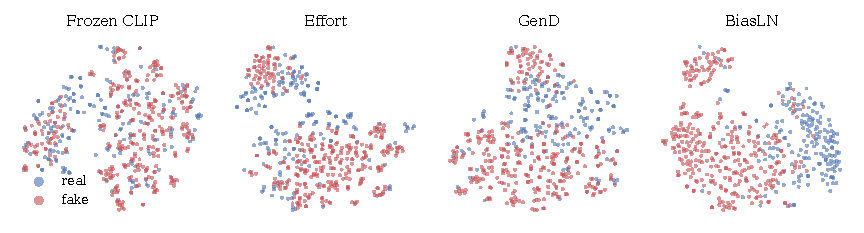
\includegraphics[width=0.85\textwidth]{generated/fig_tsne.pdf}
    \caption{T-SNE visualization of \rev{video-level} real and fake feature embeddings from \rev{the} Celeb-DF-v2 \rev{test set for the frozen CLIP encoder}, Effort, GenD and BiasLN \rev{(mean over 8 frames per video, seed 1024, checkpoints selected on FF++ validation)}.}
    \label{fig:celebdf-feature-comparison}
    \label{fig:tsne}
\end{figure*}

To compare what each model learns, we inspect the features on the Celeb-DF-v2 test set. For each \rev{video}, we \rev{average} the \rev{final class-token features of 8 frames} and map them to 2D with t-SNE. \rev{To quantify the separation independently of the projection, we also compute the Fisher ratio (between-class over within-class scatter) of the unit-normalized video features: \num{FisherClip} for the frozen encoder, \num{FisherEffort} for Effort, \num{FisherGend} for GenD and \num{FisherBiasln} for BiasLN.} As shown in Figure~\ref{fig:celebdf-feature-comparison}, BiasLN shows \rev{clearer} separation between real and fake samples than \rev{the frozen encoder}, GenD~\cite{yermakov2025gend}, and Effort~\cite{yan2025effort}. Although some overlap remains for all methods, BiasLN forms more coherent clusters, suggesting stronger representation quality on Celeb-DF-v2.

\subsection{Ablation Study}
\label{sec:ablation}
\label{sec:roles}
We conduct an ablation study to isolate the effects of parameter-efficient fine-tuning and feature normalization, as summarized in Table~\ref{tab:ablation}.
We begin with a full fine-tuning baseline using a linear classification head and cross-entropy loss, and then replace full fine-tuning with PEFT variants including LoRA~\rev{\cite{hu2022lora}}, BitFit, LayerNorm tuning, and their combination.
For LoRA, we additionally compare settings with and without $L_2$ normalization before the linear classifier to examine whether normalized features improve generalization.
All configurations are evaluated under the same protocol\rev{, share the data, schedule, loss and selection rule, and differ in one factor at a time}. The results reported in Table~\ref{tab:ablation} are video-level AUC \rev{averaged over $n$ runs with different random seeds}.

\begin{revblock}
Full fine-tuning, even with a small encoder learning rate, reaches only \num{AvgDFullft} Avg(D), far below every parameter-efficient variant: updating all weights on FF++ distorts the pre-trained features. Among the PEFT variants, BiasLN reaches \num{AvgDBiasln} Avg(D), compared with \num{AvgDBitfit} for bias-only and \num{AvgDLnLC} for LayerNorm-only tuning; these differences are within the seed-to-seed variation, as expected from Proposition~\ref{prop:fold}. Paired over seeds, BiasLN and bias-only tuning are statistically equivalent within $\pm0.01$ AUC on both averages (TOST, $p=0.002$ for Avg(D) and $p=0.019$ for Avg(M)); BiasLN is higher on Avg(D) for every seed ($+0.0018$ on average) and lower on Avg(M) ($-0.0029$), so the LayerNorm scales do not change accuracy measurably. This agrees with the analysis of Sec.~\ref{sec:analysis}: bias tuning, LayerNorm tuning and BiasLN act mainly through the same per-channel shifts, so which of them is used matters much less than adapting the frozen features at all. For LoRA, $L_2$ normalization changes Avg(D) by $-0.008$ and Avg(M) by $+0.013$ in a single run, so it is not a decisive factor either.

To see which parameters inside BiasLN matter, Table~\ref{tab:roles} further splits the tuned set. Splitting the biases by role, into the content-dependent query and fc1 biases or the residual-stream translations (value, output and fc2 biases), and tuning the LayerNorm scale or shift alone change the averages by amounts comparable with the seed-to-seed variation. No single subset is clearly better than the others, and combining all per-channel affine parameters in BiasLN gives the highest cross-dataset average in this table.
\end{revblock}

\begin{table}[H]
\centering
\captionsetup{labelsep=period, labelfont=bf, hypcap=false}
\caption{\rev{Which parameters inside BiasLN to tune ($L_2$ normalization, cross-entropy). Only the tuned subset of the encoder differs. Video AUC, mean $\pm$ std over $n$ seeds.}}
\label{tab:roles}
\resizebox{\columnwidth}{!}{% generated by tools/paper_assets.py -- do not edit
\begin{tabular}{l r c ccc}
\toprule
\textbf{Tuned parameters} & \textbf{\#} & $n$ & \textbf{Avg(D)} & \textbf{Avg(M)} & \textbf{FF++} \\
\midrule
All biases incl.\ LN $\beta$ (BitFit) & 272{,}384 & 3 & 0.921\,{\scriptsize$\pm$0.006} & 0.960\,{\scriptsize$\pm$0.005} & 0.994\,{\scriptsize$\pm$0.001} \\
$\mathbf{b}_q,\mathbf{b}_{\mathrm{fc1}}$ (content-dependent) & 122{,}880 & 1 & 0.920 & 0.958 & 0.988 \\
$\mathbf{b}_v,\mathbf{b}_o,\mathbf{b}_{\mathrm{fc2}}$ (translations) & 73{,}728 & 1 & 0.915 & 0.960 & 0.993 \\
LN $\gamma,\beta$ & 51{,}200 & 1 & 0.921 & 0.959 & 0.987 \\
LN $\beta$ only & 25{,}600 & 1 & 0.914 & 0.958 & 0.985 \\
LN $\gamma$ only & 25{,}600 & 1 & 0.914 & \textbf{0.961} & 0.984 \\
BitFit + LN $\gamma$ (BiasLN) & 323{,}584 & 3 & \textbf{0.923}\,{\scriptsize$\pm$0.006} & 0.957\,{\scriptsize$\pm$0.005} & \textbf{0.995}\,{\scriptsize$\pm$0.001} \\
\bottomrule
\end{tabular}
}
\end{table}

\begin{revblock}
\subsection{Computational Cost}
\label{sec:cost}
Table~\ref{tab:cost} reports measured costs on one A100-40GB with $224\times224$ inputs. Training is forward, backward and an Adam step at batch size 32; inference latency is at batch size 1. Because bias and LayerNorm tuning change values but not the architecture, the deployed BiasLN model has exactly the cost of the frozen CLIP encoder (162 GFLOPs per image), whereas Effort and unmerged LoRA add work at every forward pass. Compared with full fine-tuning, BiasLN trains $1.42\times$ faster per step, needs 38\% less peak memory and stores an $890\times$ smaller checkpoint. Among parameter-efficient methods the training costs are similar, because back-propagation through the 24 frozen blocks dominates; the main practical savings of BiasLN are memory, storage and an unchanged inference cost.
\end{revblock}

\begin{table}[H]
\centering
\captionsetup{labelsep=period, labelfont=bf, hypcap=false}
\caption{\rev{Measured cost on an NVIDIA A100-40GB (fp32, $224\times224$). Train: batch 32, forward + backward + Adam step. Infer: batch 1. Ckpt: size of the stored trainable tensors.}}
\label{tab:cost}
\resizebox{\columnwidth}{!}{%
\begin{tabular}{l r r r r r r}
\toprule
\textbf{Method} & \textbf{Trainable} & \textbf{Ckpt} & \textbf{Train} & \textbf{Train} & \textbf{Infer} & \textbf{GFLOPs} \\
 & & \textbf{(MB)} & \textbf{img/s} & \textbf{mem (GB)} & \textbf{ms} & \\
\midrule
Linear probe & 0.002M & 0.0 & 100.6 & 1.67 & 17.0 & 162.0 \\
LayerNorm (GenD) & 0.104M & 0.4 & 47.1 & 12.16 & 17.1 & 162.0 \\
Effort & 0.199M & 0.8 & 41.7 & 13.22 & 23.8 & 162.2 \\
BitFit & 0.274M & 1.1 & 46.6 & 12.16 & 17.1 & 162.0 \\
BiasLN & 0.326M & 1.3 & 46.5 & 12.16 & 17.2 & 162.0 \\
LoRA $r{=}8$ & 0.788M & 3.0 & 45.9 & 12.87 & 18.6 & 162.4 \\
Full FT & 303.2M & 1156.7 & 32.8 & 19.72 & 17.2 & 162.0 \\
\bottomrule
\end{tabular}}
\end{table}

\section{Conclusion}

In this paper, we presented BiasLN, a generalized deepfake detection framework that follows the core intuition of Effort~\cite{yan2025effort}: a robust detector should preserve the pre-trained representation space \rev{rather than overwrite it}.
Instead of tuning the entire backbone, we update only the bias terms and LayerNorm parameters. \rev{We showed that this set is the complete per-channel affine adaptation of the encoder: LayerNorm shifts are tied bias updates, the key biases receive no gradient, and the LayerNorm scales add the only multiplicative component.}

\rev{Under a protocol that never selects checkpoints on target-domain data and reports results over seeds, BiasLN achieves the highest in-domain accuracy, cross-dataset generalization on par with re-trained GenD and cross-method generalization about one point below it, without auxiliary losses, additional modules or inference overhead. Bias tuning, LayerNorm tuning and their combination are statistically equivalent, which shows that a minimal per-channel affine adaptation of the frozen encoder already captures most of the attainable generalization.}
\rev{We also find that the checkpoint-selection rule has a large effect on cross-dataset results, and we hope that the released protocol and code help future comparisons.}
These findings highlight the importance of preserving pre-trained representations while keeping the adaptation simple, and they support the practical value of parameter-efficient designs for robust deepfake detection.

\section{Limitations and Future Work}
\label{sec:limits}
Although our method \rev{is competitive with} current state-of-the-art methods on the benchmark, it still has several limitations that should be addressed in future work.

\rev{First, all models are trained on FF++ only, and checkpoints are selected on its in-domain validation split. A validation mixture built from datasets that are not used for testing could select better checkpoints without leaking test information.}

Second, our model works on cropped video frames instead of full video sequences.
Because of this, the model may miss temporal inconsistencies and motion artifacts that only appear across consecutive frames.

\rev{Third, the cross-method evaluation covers seven face-swapping methods of DF40; entire-face synthesis and diffusion-based editing are not evaluated, and the evaluation relies on pre-processed, face-cropped public benchmarks rather than full videos under real operating conditions (variable acquisition, compression and adversarial post-processing).}

\rev{Fourth, the CLIP ViT-L/14 backbone requires 162 GFLOPs per image, so deployment on edge devices would require distilling the detector into a smaller encoder.} Strong results on public benchmarks also do not eliminate the risk of misuse. As deepfake detectors become more effective, malicious users may use their feedback to create more realistic fake content.

In future work, we will study better validation strategies, such as building a mixed validation set from multiple datasets. We also plan to incorporate temporal modeling for video-level artifacts, evaluate the method on newer manipulation techniques, and examine how it can be deployed more safely in practice.

\begin{thebibliography}{99}
\balance

\bibitem{goodfellow2020gan}
Goodfellow I, Pouget-Abadie J, Mirza M, Xu B, Warde-Farley D, Ozair S, Courville A, Bengio Y.
Generative adversarial networks.
Commun ACM. 2020;63(11):139--44.

\bibitem{yang2022diffusion}
Yang L, Zhang Z, Song Y, Hong S, Xu R, Zhao Y, Zhang W, Cui B, Yang MH.
Diffusion models: A comprehensive survey of methods and applications.
ACM Comput Surv. 2023;56(4):1--39. doi:10.1145/3626235.

\bibitem{radford2021clip_vitl}
Radford A, Kim JW, Hallacy C, Ramesh A, Goh G, Agarwal S, et al.
Learning transferable visual models from natural language supervision.
In: Proc Int Conf Mach Learn (ICML). 2021;8748--63.

\bibitem{caron2021emerging}
Caron M, Touvron H, Misra I, J{\'e}gou H, Mairal J, Bojanowski P, Joulin A.
Emerging properties in self-supervised vision transformers.
In: Proc IEEE/CVF Int Conf Comput Vis (ICCV). 2021.

\bibitem{ojha2023universal}
Ojha U, Li Y, Lee YJ.
Towards universal fake image detectors that generalize across generative models.
In: Proc IEEE/CVF Conf Comput Vis Pattern Recognit (CVPR). 2023;24480--9.

\bibitem{kumar2022finetuning}
Kumar A, Raghunathan A, Jones R, Ma T, Liang P.
Fine-tuning can distort pretrained features and underperform out-of-distribution.
In: Int Conf Learn Represent (ICLR). 2022.

\bibitem{yan2025effort}
Yan Z, Wang J, Jin P, Zhang KY, Liu C, Chen S, et al.
Orthogonal subspace decomposition for generalizable AI-generated image detection.
In: Proc Int Conf Mach Learn (ICML). 2025.

\bibitem{yermakov2025gend}
Yermakov A, Cech J, Matas J, Fritz M.
Deepfake detection that generalizes across benchmarks.
In: Proc IEEE/CVF Winter Conf Appl Comput Vis (WACV). 2026;773--83.

\bibitem{benzaken2022bitfit}
Ben Zaken E, Goldberg Y, Ravfogel S.
BitFit: Simple parameter-efficient fine-tuning for transformer-based masked language models.
In: Proc 60th Annu Meet Assoc Comput Linguist (ACL), Vol 2. 2022;1--9.

\bibitem{wang2022ln}
Qi W, Ruan YP, Zuo Y, Li T.
Parameter-efficient tuning on layer normalization for pre-trained language models.
arXiv preprint arXiv:2211.08682. 2022.

\bibitem{yan2023deepfakebench}
Yan Z, Zhang Y, Yuan X, Lyu S, Wu B.
DeepfakeBench: A comprehensive benchmark of deepfake detection.
Adv Neural Inf Process Syst (NeurIPS), Datasets and Benchmarks Track. 2023;36:4534--65.

\bibitem{yan2024df40}
Yan Z, Yao T, Chen S, Zhao Y, Fu X, Zhu J, Luo D, Wang C, Ding S, Wu Y, Yuan L.
DF40: Toward next-generation deepfake detection.
Adv Neural Inf Process Syst (NeurIPS), Datasets and Benchmarks Track. 2024.

\bibitem{yan2023ucf}
Yan Z, Zhang Y, Fan Y, Wu B.
UCF: Uncovering common features for generalizable deepfake detection.
In: Proc IEEE/CVF Int Conf Comput Vis (ICCV). 2023.

\bibitem{yan2024latent}
Yan Z, Luo Y, Lyu S, Liu Q, Wu B.
Transcending forgery specificity with latent space augmentation for generalizable deepfake detection.
In: Proc IEEE/CVF Conf Comput Vis Pattern Recognit (CVPR). 2024.

\bibitem{rossler2019ff}
R{\"o}ssler A, Cozzolino D, Verdoliva L, Riess C, Thies J, Nie{\ss}ner M.
FaceForensics++: Learning to detect manipulated facial images.
In: Proc IEEE/CVF Int Conf Comput Vis (ICCV). 2019.

\bibitem{qian2020frequency}
Qian Y, Yin G, Sheng L, Chen Z, Shao J.
Thinking in frequency: Face forgery detection by mining frequency-aware clues.
In: Proc Eur Conf Comput Vis (ECCV). 2020.

\bibitem{hu2022lora}
Hu EJ, Shen Y, Wallis P, Allen-Zhu Z, Li Y, Wang S, et al.
LoRA: Low-rank adaptation of large language models.
In: Int Conf Learn Represent (ICLR). 2022.

\bibitem{wang2020alignment}
Wang T, Isola P.
Understanding contrastive representation learning through alignment and uniformity on the hypersphere.
In: Proc Int Conf Mach Learn (ICML). 2020.

\bibitem{namazifar2023bias}
Namazifar M, Hazarika D, Hakkani-T{\"u}r D.
Role of bias terms in dot-product attention.
In: Proc IEEE Int Conf Acoust Speech Signal Process (ICASSP). 2023.

\bibitem{giannou2023layernorm}
Giannou A, Rajput S, Papailiopoulos D.
The expressive power of tuning only the normalization layers.
In: Proc Conf Learn Theory (COLT). 2023.

\bibitem{valizadeh2024layernorm}
ValizadehAslani T, Liang H.
LayerNorm: A key component in parameter-efficient fine-tuning.
arXiv preprint arXiv:2403.20284. 2024.

\bibitem{xu2026bpl}
Xu Y, He R, Yan Z, Dong Y, Han Z, Wang X, Yin Y.
BPL: Generalizable deepfake detection via bias-only pair-aware learning.
In: Proc Int Conf Mach Learn (ICML). 2026.

\bibitem{deng2020retinaface}
Deng J, Guo J, Ververas E, Kotsia I, Zafeiriou S.
RetinaFace: Single-shot multi-level face localisation in the wild.
In: Proc IEEE/CVF Conf Comput Vis Pattern Recognit (CVPR). 2020.

\bibitem{liu2021spsl}
Liu H, Li X, Zhou W, Chen Y, He Y, Xue H, et al.
Spatial-phase shallow learning: Rethinking face forgery detection in frequency domain.
In: Proc IEEE/CVF Conf Comput Vis Pattern Recognit (CVPR). 2021.

\bibitem{luo2021srm}
Luo Y, Zhang Y, Yan J, Liu W.
Generalizing face forgery detection with high-frequency features.
In: Proc IEEE/CVF Conf Comput Vis Pattern Recognit (CVPR). 2021.

\bibitem{ni2022core}
Ni Y, Meng D, Yu C, Quan C, Ren D, Zhao Y.
CORE: Consistent representation learning for face forgery detection.
In: Proc IEEE/CVF Conf Comput Vis Pattern Recognit Workshops (CVPRW). 2022.

\bibitem{cao2022recce}
Cao J, Ma C, Yao T, Chen S, Ding S, Yang X.
End-to-end reconstruction-classification learning for face forgery detection.
In: Proc IEEE/CVF Conf Comput Vis Pattern Recognit (CVPR). 2022.

\bibitem{chen2022sladd}
Chen L, Zhang Y, Song Y, Liu L, Wang J.
Self-supervised learning of adversarial example: Towards good generalizations for deepfake detection.
In: Proc IEEE/CVF Conf Comput Vis Pattern Recognit (CVPR). 2022.

\bibitem{shiohara2022sbi}
Shiohara K, Yamasaki T.
Detecting deepfakes with self-blended images.
In: Proc IEEE/CVF Conf Comput Vis Pattern Recognit (CVPR). 2022.

\bibitem{huang2023iid}
Huang B, Wang Z, Yang J, Ai J, Zou Q, Wang Q, Ye D.
Implicit identity driven deepfake face swapping detection.
In: Proc IEEE/CVF Conf Comput Vis Pattern Recognit (CVPR). 2023.

\bibitem{cheng2024prodet}
Cheng J, Yan Z, Zhang Y, Luo Y, Wang Z, Li C.
Can we leave deepfake data behind in training deepfake detector?
Adv Neural Inf Process Syst (NeurIPS). 2024.

\bibitem{lin2024cdfa}
Lin Y, Song W, Li B, Li Y, Ni J, Chen H, Li Q.
Fake it till you make it: Curricular dynamic forgery augmentations towards general deepfake detection.
In: Proc Eur Conf Comput Vis (ECCV). 2024. doi:10.1007/978-3-031-73016-0\_7.

\bibitem{cui2025forada}
Cui X, Li Y, Luo A, Zhou J, Dong J.
Forensics Adapter: Adapting CLIP for generalizable face forgery detection.
In: Proc IEEE/CVF Conf Comput Vis Pattern Recognit (CVPR). 2025;19207--17.

\bibitem{badr2025wavit}
Badr NEA, Nebel JC, Greenhill D, Liang X.
WaViT-CDC: Wavelet vision transformer with central difference convolutions for spatial-frequency deepfake detection.
IEEE Open J Signal Process. 2025;6:621--30. doi:10.1109/OJSP.2025.3571679.

\bibitem{li2020celeb}
Li Y, Yang X, Sun P, Qi H, Lyu S.
Celeb-DF: A large-scale challenging dataset for deepfake forensics.
In: Proc IEEE/CVF Conf Comput Vis Pattern Recognit (CVPR). 2020;3207--16.

\bibitem{dufour2019dfd}
Dufour N, Gully A.
Contributing data to deepfake detection research.
Google Research Blog. 2019. Available from: \url{https://research.google/blog/contributing-data-to-deepfake-detection-research/}.

\bibitem{dolhansky2019dfdcp}
Dolhansky B, Howes R, Pflaum B, Baram N, Ferrer CC.
The deepfake detection challenge (DFDC) preview dataset.
arXiv preprint arXiv:1910.08854. 2019.

\bibitem{dolhansky2020dfdc}
Dolhansky B, Bitton J, Pflaum B, Lu J, Howes R, Wang M, Ferrer CC.
The DeepFake Detection Challenge (DFDC) dataset.
arXiv preprint arXiv:2006.07397. 2020.

\end{thebibliography}

\end{document}
